\documentclass[a4paper]{article}
\usepackage[spanish]{babel}
\usepackage[utf8]{inputenc}
\usepackage{charter}   % tipografia
\usepackage{graphicx}
%\usepackage{makeidx}
\usepackage{paralist} %itemize inline

\usepackage{color} % para snipets de codigo coloreados
\usepackage{fancybox}  % para el sbox de los snipets de codigo

\definecolor{litegrey}{gray}{0.94}

% \newenvironment{sidebar}{%
% 	\begin{Sbox}\begin{minipage}{.85\textwidth}}%
% 	{\end{minipage}\end{Sbox}%
% 		\begin{center}\setlength{\fboxsep}{6pt}%
% 		\shadowbox{\TheSbox}\end{center}}
% \newenvironment{warning}{%
% 	\begin{Sbox}\begin{minipage}{.85\textwidth}\sffamily\lite\small\RaggedRight}%
% 	{\end{minipage}\end{Sbox}%
% 		\begin{center}\setlength{\fboxsep}{6pt}%
% 		\colorbox{litegrey}{\TheSbox}\end{center}}

\newenvironment{codesnippet}{%
	\begin{Sbox}\begin{minipage}{\textwidth}\sffamily\small}%
	{\end{minipage}\end{Sbox}%
		\begin{center}%
		\vspace{-0.4cm}\colorbox{litegrey}{\TheSbox}\end{center}\vspace{0.3cm}}




\usepackage{fancyhdr}

\pagestyle{fancy}

\renewcommand{\sectionmark}[1]{\markright{\thesection\ - #1}}

\fancyhf{}

\fancyhead[LO]{Sección \rightmark} % \thesection\ 
\fancyfoot[LO]{\small{Leandro Raffo, Maximiliano Fernández Wortman, Uriel Rozenberg.}}
\fancyfoot[RO]{\thepage}

\renewcommand{\headrulewidth}{0.5pt}
\renewcommand{\footrulewidth}{0.5pt}
\setlength{\hoffset}{-1.1in}
\setlength{\textwidth}{18cm}
%\setlength{\hoffset}{-1.1cm}
%\setlength{\textwidth}{16cm}
\setlength{\headsep}{0.5cm}
\setlength{\textheight}{25cm}
\setlength{\voffset}{-0.7in}
\setlength{\headwidth}{\textwidth}
\setlength{\headheight}{13.1pt}

\renewcommand{\baselinestretch}{1.1}  % line spacing




% \setcounter{secnumdepth}{2}

\usepackage{caratula}


\begin{document}


\thispagestyle{empty}
\materia{Organización del Computador II}
\submateria{Segundo Cuatrimestre de 2015}
\titulo{Trabajo Práctico II}
\subtitulo{Programacion SIMD}
\integrante{Leandro Raffo}{}{}
\integrante{Maximiliano Fernández Wortman}{}{}
\integrante{Uriel Rozenberg}{}{}

%Pagina de titulo e indice
%\thispagestyle{empty}

\maketitle 

\tableofcontents

\newpage

\section{Introduccion}
En este trabajo práctico realizamos la implementación de dos filtros de imagenes, con tal de ver que tan eficiente puede llegar a ser (o no) SIMD, los filtros son la diferencia de imagenes y el blur gaussiano, los cuales fueron implementados en lenguaje C (gcc y clang) y assembly, haciendo uso de instrucciones vectoriales. Luego comparamos la performance de estas implementaciones sobre diferentes imagenes y usando herramientas probabilísticas y estadísticas.

\section{Implementacion}

\subsection{Diferencia}
\noindent Descripcíon de un ciclo de la iteración del filtro diferencia.\\
Primermo pedimos memoria para declarar las máscaras que vamos a usar y armamos el stackframe (omitido)
\begin{codesnippet}
\begin{verbatim}
section .rodata
mascara_copia_pixels db 2,2,2,2,6,6,6,6,10,10,10,10,14,14,14,14
mascara_asigna_alpha db 0,0,0,255,0,0,0,255,0,0,0,255,0,0,0,255
\end{verbatim}
\end{codesnippet}

\noindent Luego de armar el stackframe tenemos
\begin{codesnippet}
\begin{verbatim}
mov r12, rdx
mov eax, r8d
mov ecx, ecx
mul rcx
xor r15, r15
\end{verbatim}
\end{codesnippet}
r12 apunta a la matriz resultado, ecx tiene la cantidad de filas, y la parte baja de rax(eax) tiene la cantidad de columnas. Al hacer mul rcx se tiene filas*columnas en rdx:rax, como movimos cosas de 32 bits obtenemos la multiplicación en rax, que es lo que vamos a usar, junto a r15 para iterar (notar que tenemos en cuenta para esto que los movimientos de registros entre dwords limpian la parte alta de los registros de 64bits, es decir extendemos el número usando que son enteros positivos). Ahora entramos al ciclo.

\begin{codesnippet}
\begin{verbatim}
.ciclo:
    cmp r15, rax
    JE .fin
\end{verbatim}
\end{codesnippet}

\noindent Comparamos si r15 es igual a rax en tal caso ya hicimos la diferencia sobre todos los pixeles y termina el ciclo. El ciclo sigue con

\begin{codesnippet}
\begin{verbatim}
    movdqu xmm3 , [RDI +  r15*4]   
    movdqu xmm15, [RSI +  r15*4]
    movdqu xmm14, xmm15     
    pminub xmm15, xmm3        
    pmaxub xmm3 , xmm14        
    psubb  xmm3 , xmm15             
    movdqu xmm4, xmm3 
    movdqu xmm5, xmm3       
\end{verbatim}
\end{codesnippet}

\noindent Movemos a xmm$3$ los primeros $4$ pixeles de la primera matriz y a xmm$15$ los primeros $4$ de la segunda matriz a comparar, estos ocupan respectivamente $16$ bytes en memoria (brga por $4$). Después Guardamos en xmm$14$ el valor de xmm$15$ y hacemos un pminub entre xmm$15$ y xmm$3$ lo cual deja en xmm$15$ el mínimo byte a byte. Lo mismo para xmm$3$ pero con pmaxub es decir este tiene el máximo byte a byte. Hacemos esto porque queremos calcular el valor absoluto de la forma $|x-y|$ = $\max(x,y) - \min(x,y)$. Concluimos esta idea haciendo psubb entre xmm$3$ que tenia el máximo y xmm$15$ que tenia el mínimo y finalmente guardamos el resultado en xmm$4,5$ para operar en la siguiente parte.

\begin{codesnippet}
\begin{verbatim}
    pslldq xmm4, 1                  
    pslldq xmm5, 2               
    movdqu xmm6, xmm5             
    pmaxub xmm6, xmm4             
    pmaxub xmm6, xmm3              
    pshufb xmm6, [mascara_copia_pixels] 
    paddsb xmm6, [mascara_asigna_alpha]
    movdqu [r12 +  r15*4], xmm6
    add  r15d, 4
    jmp .ciclo
\end{verbatim}
\end{codesnippet}
\noindent Ahora shifteamos con packed shift xmm$4,5$ uno y dos bytes respectivamente de forma de poder tomar el máximo de entre r g b en paralelo, es decir $4$ pixels a la vez. Por ejemplo, el primer byte de xmm$4$ tiene al byte de r, y el de xmm$6$ tiene al byte de g, de forma que al hacer pmaxub entre  xmm$6$ y xmm$4$ nos deja en el primer byte de xmm$6$ (y cada 3 bytes) max(r$_n$,g$_n$) donde $n = \{1,2,3,4 \}$ indican los pixeles que levantamos. Los demas bytes de este registro no nos interesan. Repetimos esto entre xmm$6$ y xmm$3$, pasa de vuelta lo mismo pero ahora tenemos en el primer byte de xmm$6$ (y cada $3$ bytes) max(r$_n$,g$_n$,b$_n$) con $n = \{1,2,3,4 \}$. Ahora tenemos que mover este máximo a las 3 coordenadas r, g y b, hacemos esto mediante la mascara mask$_5$ y mediante trans$_2$ sumamos con saturación con tal de dejar en alpha el valor $255$. Copiamos los 16 bytes correspondientes (con el offset adecuado) en la matriz destino, sumamos $4$ a r$15$d y saltamos para, si es necesario, volver a hacer el ciclo completo.


\subsection{Blur gaussiano}

\noindent El blur gaussiano consta de dos ciclos uno anidado sobre el otro, el anidado itera sobre el kernel y el que anida itera sobre la matriz, usamos SIMD para hacer los calculos sobre un pixel en simultaneo (es decir las 4 componentes rgba a la vez), además en vez de hacer offsets para atras como el codigo en C nos movemos siempre para adelante, por ejemplo, empezamos en el pixel $0$ y recorremos la submatriz que va de $0, 2r$ en filas y $0, 2r$ en columnas, donde $r$ es el radio, a la par de la matriz del kernel (que también tiene este tamaño) haciendo las multiplicaciones y acumulandolas, luego cuando terminamos de iterar sobre el kernel, insertamos en el pixel destino, que esta en la posición ($r, r$), luego aumentamos la columna y seguimos este proceso hasta el ancho $- 2r$ donde nos paramos en la proxima fila y repetimos hasta llegar a la altura $- 2r$, es decir siempre que insertamos el pixel estamos en rango. Ahora pasamos a describir más en detalle las operaciones que usamos para esto.\\
\noindent Antes de entrar al ciclo preparamos algunos registros para saber hasta donde iterar, tenemos que: rax guarda el último valor hasta el que vamos a recorrer que es igual a  [(filas $- 2r$)*columnas] $-2r$, rbp va a guardar hasta donde vamos a hacer cada subciclo es decir $(2r+1)^2$, r11 tiene el valor $2r$, r12 la matriz fuente, r13 la matriz destino, r8 la cantidad de columnas y rbx (ebx) el offset necesario para insertar el pixel en la matriz destino.
\begin{codesnippet}
\begin{verbatim}
.ciclo_kernel:
    cmp rcx, rbp                      
    je .insert          
    mov r9, rsi
    add r9, rdi
    movd        xmm0, [ r12 + r9 ]      
    punpcklbw   xmm0, xmm8              
    punpcklwd   xmm0, xmm8              
    cvtdq2ps    xmm0, xmm0              
    movd        xmm1, [ r10 + rcx*4 ]   
    movq        xmm3, xmm1              
    pslldq      xmm3, 4
    paddd       xmm3, xmm1              
    pslldq      xmm3, 4
    paddd       xmm3, xmm1                           
    mulps       xmm0, xmm3              
    addps       xmm2, xmm0              

\end{verbatim}
\end{codesnippet}

\noindent Primero verificamos si tenemos que insertar el pixel, para esto comparamos rcx, el registro que cuenta sobre el tamaño del kernel contra rbp que mantenia hasta donde teniamos que iterar para haber recorrido el kernel, si no, levantamos de memoria un pixel (double word) con la operacion movd, rsi itera sobre la matriz fuente/destino y rdi itera la columna del kernel, rcx itera el kernel linealmente, y lo guardamos en xmm0, xmm8 está previamente con el valor $0$ y lo vamos a usar para desempaquetar los $4$ bytes. Desempaquetamos primero a words, es decir tenemos que los bytes son la parte baja de un word y la parte alta esta llena de $0$s. Repetimos pero con double word y convertimos a float empaquetado. Ahora movemos el valor de la matriz de convolución con movd (un float por eso el *$4$) a xmm1, shifteamos 4 bytes con pslldq movemos un quadword shifteamos y hacemos un packed add (queremos copiar el valor del float) shifteamos xmm3 y volvemos a sumar una vez más, para que cada doubleword de xmm3 tenga el flaot. Ahora multiplicamos el float de xmm3 contra los valores del pixel que desempaquetamos en xmm0 dejando en xmm0 este valor y lo acumulamos en xmm2.

\begin{codesnippet}
\begin{verbatim}
    cmp rdx, r11
    je .sumar_fila_kernel
    add rdx, pixel_size
    inc rcx
    add rsi, pixel_size
    jmp .ciclo_kernel
\end{verbatim}
\end{codesnippet}
rdx mantiene el contador para iterar sobre la fila, si este es igual a 2r saltamos a sumar\_fila\_kernel de lo contrario adelantamos rdx y rsi en pixel\_size (que es un \%define con el valor $4$) y entramos al ciclo de vuelta.


\begin{codesnippet}
\begin{verbatim}
.sumar_fila_kernel:
    xor rdx, rdx
    sub rsi, r11                      
    add rsi, r8                        
    inc rcx
    jmp .ciclo_kernel
\end{verbatim}
\end{codesnippet}


\noindent En sumar fila limpiamos rdx, para volver a poder iterar de $0$ a $2r$, le restamos $2r$ a rsi, este iteraba sobre la fila para la matriz mas grande y le sumamos al mismo la cantidad de columnas, es decir rsi apunta al comienzo de la fila siguiente, incrementamos rcx asi en el proximo ciclo apunta a la siguiente fila tambien y saltamos al ciclo de vuelta.

\begin{codesnippet}
\begin{verbatim}
 .insert:
    pxor     xmm4, xmm4
    cvtps2dq xmm2, xmm2                 
    packusdw xmm2, xmm4                 
    packuswb xmm2, xmm4                 
    movd     xmm7, ebx
    add      rbx, rdi
    movd     [ r13 + rbx ], xmm2           
    movd     ebx, xmm7
    pxor     xmm7, xmm7
    xor rsi, rsi
    xor rcx, rcx
    cmp rdi, r15
    je .sumar_fila
    add rdi, pixel_size
    jmp .ciclo_matriz
\end{verbatim}
\end{codesnippet}

En .insert hacemos casi lo contrario a levantar, convertimos los floats empaquetados que estaban en xmm2 a doublewords empaquetados y re-empaquetamos a word y luego a byte. Luego sumamos rbx e rdi para obtener la posición en la que vamos a insertar el pixel (los 4 bytes) e insertamos el pixel. Una vez que esto pasa ponemos rsi y rcx en $0$ y vemos si llegamos a la ultima columna que teniamos que iterar, si pasa esto saltamos a sumar\_fila sino sumamos pixel\_size a rdi y saltamos al ciclo del kernel de vuelta.

\begin{codesnippet}
\begin{verbatim}
.sumar_fila:
    add rdi, r11                 
    add r15, r8                    
    jmp .ciclo_matriz
\end{verbatim}
\end{codesnippet}

\noindent En .sumar\_fila lo que hacemos es sumarle a rdi lo que faltaba para llegar a la proxima columna, $2r$ y le sumamos a r15 la cantida de columnas, r15 en este caso mantiene (acorde al rdi) hasta que columna tenemos que iterar. Basicamente r15 empieza en cols $-2r$ y se le van sumando el total de columnas, en la segunda iteracion tiene $2$cols $-2r$ etc. Aca saltamos a ciclo\_matriz y no ciclo\_kernel, este contiene lo siguiente.

\begin{codesnippet}
\begin{verbatim}
.ciclo_matriz:
    cmp rdi, rax                       
    jg .end
\end{verbatim}
\end{codesnippet}

\noindent Si rdi es mayor que rax (que marcaba el ultimo pixel sobre el que podiamos iterar) saltamos al final, desarmamos el stackframe y retornamos.

\section{Resultados}

\subsection{Diferencia}

\noindent \textbf{Nota:} todos los tests fueron corridos sobre una PC con procesador Intel Core2Duo E8440.
\\
\noindent Para analizar las implementaciones de C y assembly, corrimos 1000 iteraciones de cada implementación de diferencia sobre una imagen de 2308x2308 (16mb) donde las implementaciones de C se compilaron con gcc y clang usando los flags de optimización -O0, -O1, -O2, -O3 y -Os. Basicamente los flags de -O\# con \# un número entre $0,3$ intentan optimizar principalmente para velocidad y luego tamaño, $0$ siendo el menos 'optimizado' y $3$ el más optimizado, mientras que -Os optimiza principalmente por tamaño del ejecutable, algunas cosas notables son que por ejemplo (luego de hacer un disassembly) notamos que a partir de -O2 gcc ya no armaba un stackframe, ni resguardaba rbp, y pusheaba a medida que necesitaba los registros, alineando rsp cuando fuese necesario, diferencias observables entre -O2 y -O3 fue el uso de operaciones SIMD, por ejemplo de empaquetado y desempaquetado, multiplicaciones packed etc en -O3 (para el blur), mientras que esto no pasaba en -O2, extrañamente la performance es la misma y tal vez se debe a otros factores como el modelo de procesador (Intel c2d E840). Se adjuntan los objdump del build en distintas optimizaciones. \newline


\noindent A continuación dejamos los gráfico con el promedio (con y sin outliers) de la diferencia bajo distintos flags de optimización y en assembly.
 \newpage
 
\begin{figure}[h]
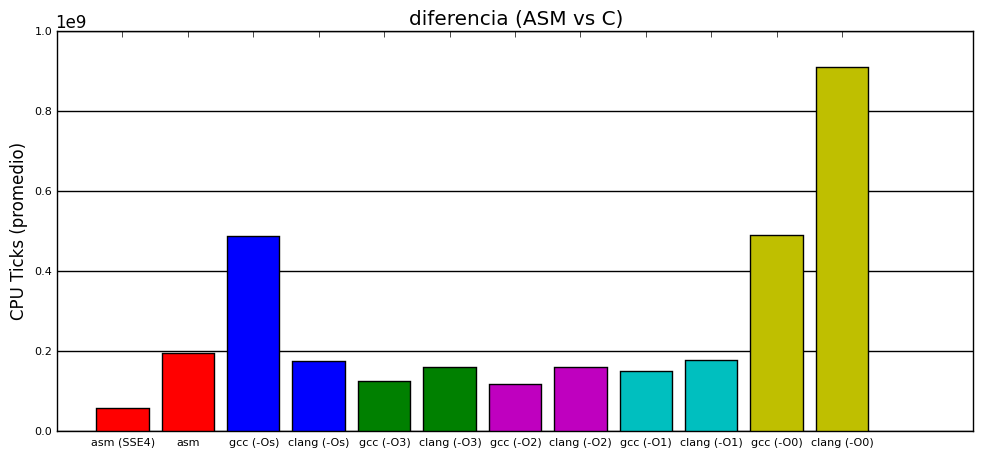
\includegraphics[scale=0.71]{imagenes/test_difrencia_ASM_C_PROMEDIO_Os}
\caption{Promedio, 1000 iteraciones sobre una imagen de 2308x2308 pixels de 16mb.}
\end{figure}

Como podemos observar, la versión en assembler usando instrucciones vectorizadas es más de dos veces mas rapida que cualquiera de las otras implementaciones. En particular es 



\newpage 

\noindent En el siguiente experimento queria ver si el tamaño de la imagen iba a modificar la performance (incrementar el tiempo de ejecucion) del algoritmo debido a cache misses. Para esto corrimos diferencia en Assembly y C, de vuelta bajo gcc y clang, pero esta vez con el flag -O2, ya que me parecio que era el sweet spot para esta implementación ya que los flags de optimización no garantizan que corra con mejor performance, sobre imágenes que iban de 256kb a 64mb como se ve en la figura (Los tamaños utilizados están en el shellscript convertir.sh que es el que usamos para generar las imagenes). 

\begin{figure}[h]
	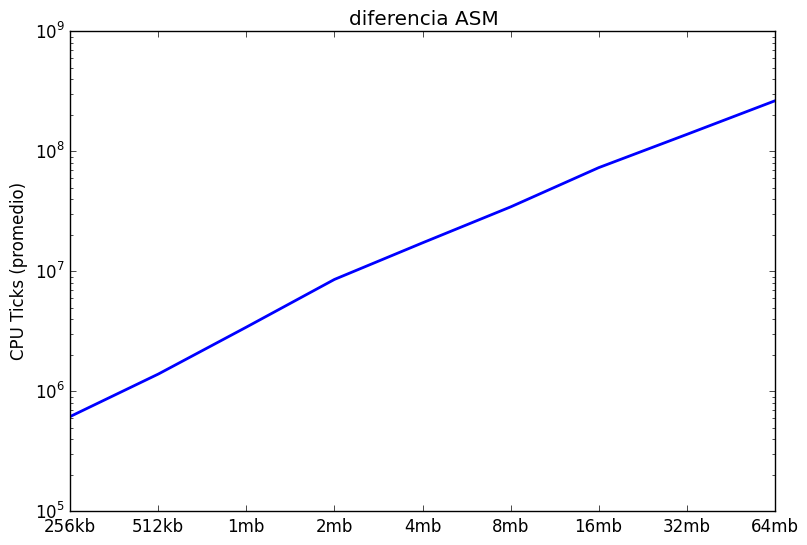
\includegraphics[scale=0.60]{imagenes/test_performance_size_ASM.png}
	\caption{Diferencia en asm, escala logarítmica}
\end{figure}

\noindent Lo que se obtuvo es una curva que sube suavemente, lo cual implicaria que el algoritmo tiene un crecimiento bastante predecible hasta el tamaño donde se lo probó (imágenes de 4000x4000 pixels con un tamaño de 64mb).

\begin{figure}[h]
	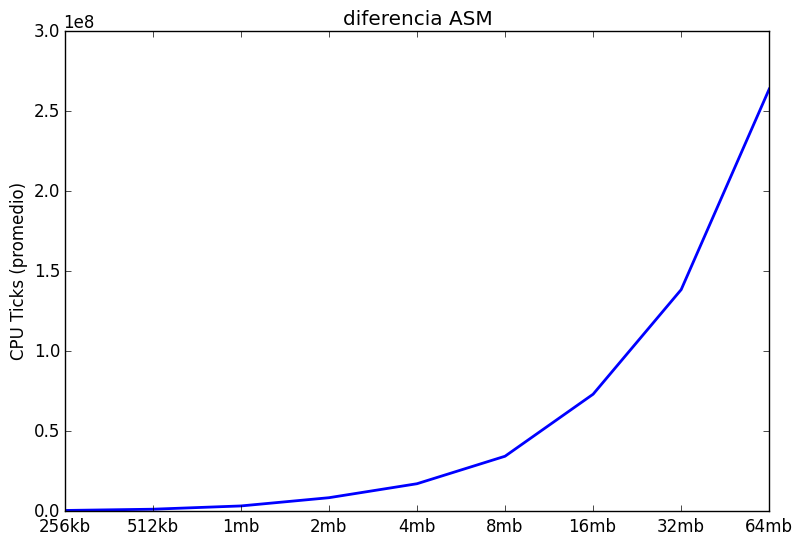
\includegraphics[scale=0.60]{imagenes/test_performance_size_ASM_not_log.png}
	\caption{Diferencia en asm, escala no logarítmica}
\end{figure}

\newpage 

Lo mismo pasa con las implementaciones en C, en este caso gcc con -O2.

\begin{figure}[h]
	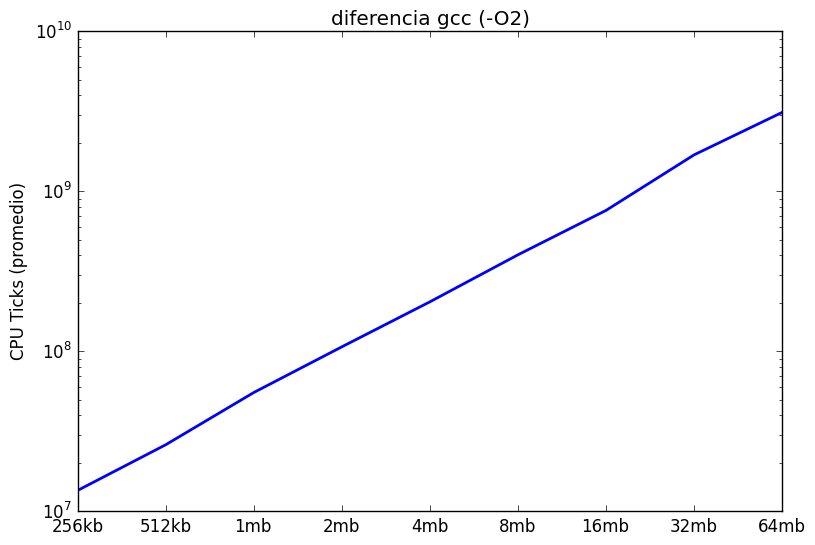
\includegraphics[scale=0.60]{imagenes/test_performance_size_C.png}
	\caption{Diferencia en C, escala logarítmica}
\end{figure}


\subsection{Blur}

\noindent Una de las hipótesis que teniamos con blur es que dada una imagen con un radio pequeño iba a correr mas lento que con un radio mas grande, pero a medida que el radio domine la cantidad de pixeles sobre las cuales va a aplicar la matriz de convolución el tiempo de ejecución iba a bajar. Esto lo pudimos probar corriendo blur sobre una imagen de tamaño fijo (en este caso 584x584 pixels) e incrementando el radio como se ve en la siguiente imagen

\begin{figure}[h]
	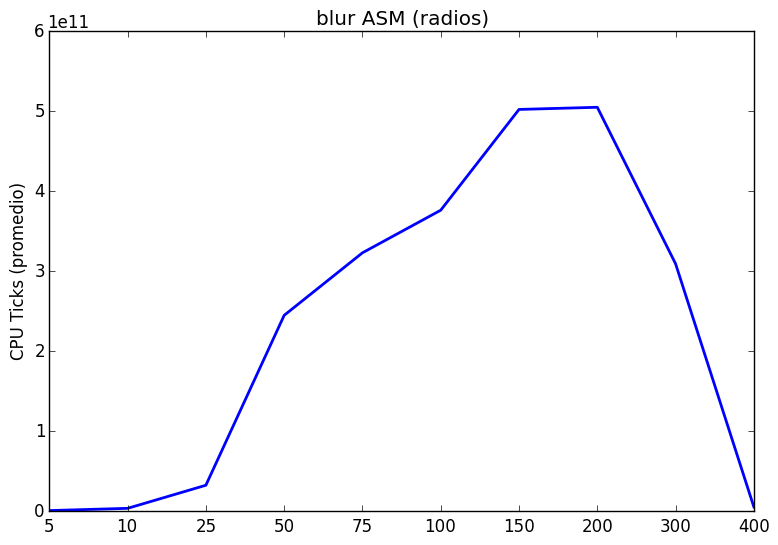
\includegraphics[scale=0.62]{imagenes/test_radio_size_ASM.png}
	\caption{Blur, cambiando los radios}
\end{figure}

El algoritmo llega a un punto crítico cuando el radio es equivalente a la dimensión/2, es decir cuando el algoritmo se comporta como $O(n^4)$ sobre la dimensión.


\newpage 

Para comparar al algoritmo en C vs asm hicimos lo mismo que blur, corrimos los dos sobre la misma imagen y calculamos su promedio.


\begin{center}
    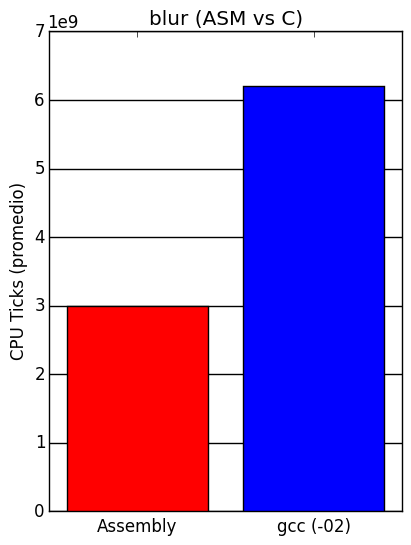
\includegraphics[scale=0.6]{imagenes/test_blur_ASM_C.png}
\end{center}

\section{Conclusión}

\noindent Para el algoritmo de diferencia, se justificaria totalmente hacer una implementación en SIMD, no solo por el hecho de que corre mas rápido, sino que además implementarlo en assembly fue bastante fácil ($<$ 20 lineas). 

\end{document}
